\documentclass{article}
\usepackage[a4paper]{geometry}
\usepackage{xskak,chessboard}
\usepackage[ngerman]{babel}
\usepackage{fancyhdr,hyperref,multicol,caption,float}



\pagestyle{fancy}
\fancyhf{}
\lhead{Wahlfachwoche 2024}
\rhead{
\includegraphics[width=2cm]{Logo-GYM-Muttenz}}
%\cfoot{Seite \thepage}
%\lfoot{Fa, DC}

%\title{Schach 1.0}
%\author{Daniel Fasnacht, Oliver De Capitani}
%\subtitle{Wahlfachwoche 2019}
%\date{24.-28. Juni 2019}

\parindent=0mm


\renewcommand{\arraystretch}{1.2}

\begin{document}
\setchessboard{showmover=false}

%\vspace*{0.5cm}
%\section*{Schach -- Das Königliche Spiel}
%{\bf Projekt Wahlfachwoche 2021 (28.Juni - 2. Juli 2021)}
%
%{\bf Veranstaltende Lehrpersonen:} Matthias Bürgin, Oliver De Capitani
%
%{\bf Kurstitel: } Schach -- Das Königliche Spiel
%
%{\bf Ziel des Kurses: } Wir werden uns eine Woche lang intensiv mit Schach beschäftigen. Wir werden Rätsel lösen, Partien spielen, Eröffnungen lernen und nnoch vieles mehr.
%
%{\bf Arbeitsweise:} Wir werden zum Teil vor Ort, zum Teil extern (''Gartenschach''); in Gruppen und einzeln and verscheidenen Themen und Probleme rund um Schach uns beschäftigen.
%
%
%
%\begin{multicols}{2}
%\begin{figure}[H]
%\centering
%\chessboard[smallboard,
%setfen=r2q1rk1/ppp3pp/2n2n2/4pbB1/8/2P2NP1/PPQ2PBP/R4RK1 w - 0 2,
%arrow=to,linewidth=0.2ex,
%pgfstyle=straightmove,
%%shortenstart=0.4em,
%color=red!80,
%markmoves={c8-f5}
%]
%\caption{Schwarz spielte gerade 1... Lf5? und wird nach 2. Dxf5 Material verlieren, da der Läufer nicht geschützt ist}
%\end{figure}
%
%\begin{figure}[H]
%\centering
%\chessboard[smallboard,
%setfen=r4rk1/3b1ppp/p1p5/1p6/4PR2/1BPn4/PP2N1PP/5R1K w - - 1 2,
%arrow=to,linewidth=0.2ex,
%pgfstyle=straightmove,
%shortenstart=0.4em,
%color=red!80,
%markmoves={f4-f7}
%]
%\caption{Der Bauer auf f7 wird dreimal angegriffen (2 Türme und ein Läufer), aber nur zweimal verteidigt. Nach 1. Txf7 wird Weiss Material gewinnen.}
%\end{figure}
%\end{multicols}


\begin{titlepage}
    \begin{center}
        \vspace*{1cm}
 
        \Huge
        \textbf{Schach 1.0}
 
        \vspace{0.5cm}
        \LARGE
        Wahlfachwoche 2025
 
        \vspace{1.5cm}
 
        \textbf{Oliver De Capitani, Simeon Jackman}
 
        \vfill
 
 
 
        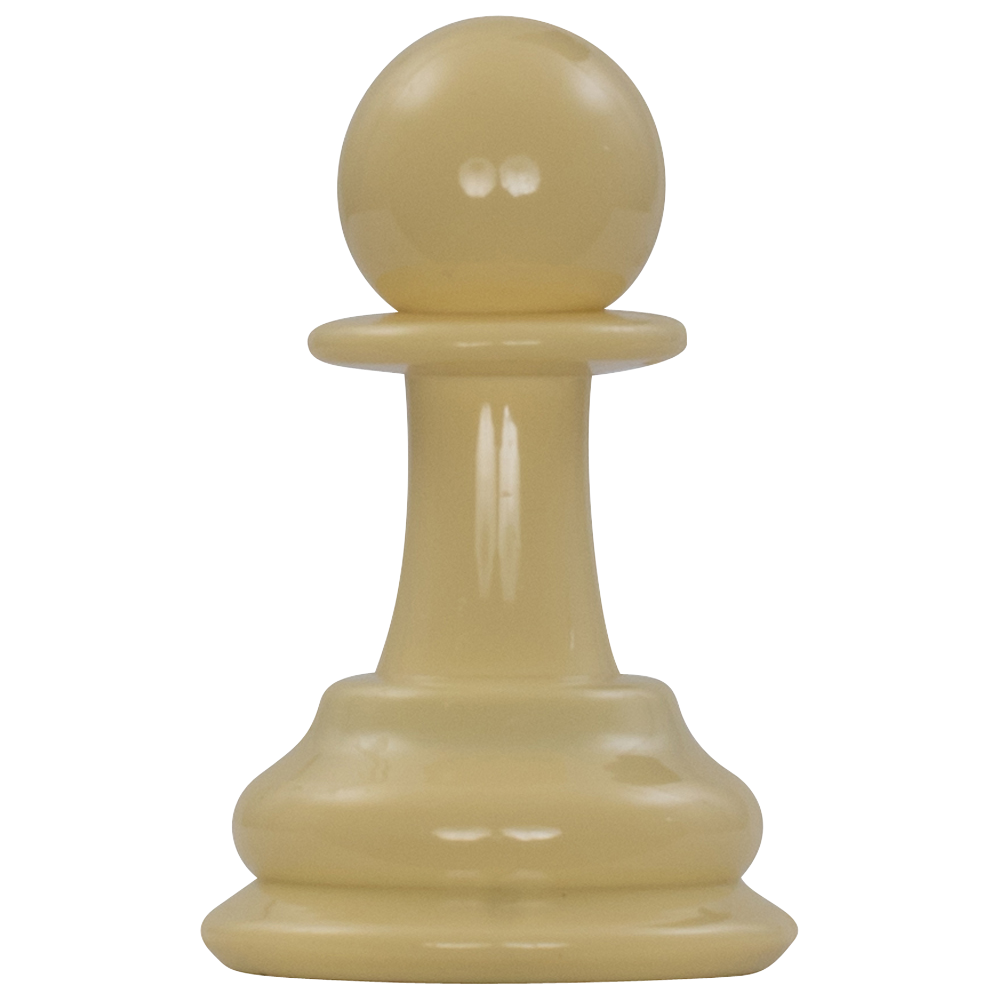
\includegraphics[width=0.6\textwidth]{pawn}
		\vfill
        
               \Large
        Gymnasium Muttenz \\
        24.6 - 28.6.2024
         
    \end{center}
\end{titlepage}

\tableofcontents

\newpage


\section{Einführung}
Schach, das königliche Spiel, hat seine Wurzeln in Indien. Irgendwann vor dem 7. Jahrhundet wurde dort das Spiel \emph{Chaturanga} entwickelt aus dem das Schach und weitere Spiele abgeleitet wurden. Im Zuge der islamischen Expansion kam das Schachspiel nach Europa, wo es im 18. und 19. Jahrhundert zu einem Spiel für die Oberschicht wurde. 

Im Laufe des 19. Jahrhunderts wurden auch die modernen Regeln des Schach festgelegt und es fanden erste Turniere statt.

Der aktuelle Weltmeister im Schach ist Ding Liren aus China.

\section{Das Schachbrett}
Das Schachbrett besteht aus 64 Felder, die quadratisch angeordnet sind. Die Felder sind abwechlungsweise schattiert. Auch wenn die Farben variieren spricht man meistens von 'schwarzen' und 'weissen' Feldern (manchmal auch 'dunkel' und 'hell'). Die einzelnen Felder sind mit "Koordinaten" beschriftet. Dabei wird zuerst die Spalte (im Schach \emph{Linie} genannt) und dann die Zeile (im Schach \emph{Reihe} genannt) angegeben:
\newchessgame

\begin{figure}[h]
\centering
\chessboard[
smallboard,
clearboard,
pgfstyle=border,
color=red,
linewidth=0.1ex,
markfield=e4
]
\caption{Das Schachbrett -- das Feld $e4$ ist markiert}
\end{figure}

Teilweise werden auch relative Positionen angegeben: Die Reihe 1 ist die \emph{Grundreihe} für Weiss; die Reihe 8 ist die \emph{Grundreihe} für Schwarz.

\newpage

\section{Die Figuren und wie sie Ziehen}
\subsection{Der König}

\begin{multicols}{2}
Der König ist die wichtiste Figur im Schach. Ihn gilt es zu schützen -- um jeden Preis. Der König darf nur ein Feld weit ziehen und schlagen; das aber dafür in jede Richtung. Die Ausnahme bildet die Rochade ($\rightarrow$ \hyperref[rochade]{Rochade}).

Zu Beginn ist der König eine schwache Figur und muss beschütrtzt werden, aber im Endspiel ist es wichtig den  König zu aktivieren. 
\vfill\null
\columnbreak
\begin{figure}[H]
\centering
\chessboard[
smallboard,
setpieces={Ke4},
arrow=to,linewidth=0.2ex,
pgfstyle=straightmove,
shortenstart=0.4em,
color=red!80,
markmoves={e4-e5,e4-d5,e4-d4,e4-d3,e4-e3,e4-f3,e4-f4,e4-f5},
%pgfstyle=border,
%color=red,
%linewidth=0.1ex,
%markfields={e5,d5,d4,d3,e3,f3,f4,f5}
]
\caption{Die Züge des Königs}
\end{figure}
\end{multicols}


\subsection{Die Dame}
\begin{multicols}{2}
Die Dame ist wohl die mächtigste Figur im Schach. Wie der König darf sie in jede Richtung ziehen und schlagen -- aber beliebig weit.

Die Dame sollte zu Beginn nicht zu weit vorpreschen; ansonsten kann es sein, dass sie irgendwo 'eingekesselt' wird.
\vfill\null
\columnbreak
\begin{figure}[H]
\centering
\chessboard[
smallboard,
setpieces={Qe4},
arrow=to,linewidth=0.2ex,
pgfstyle=straightmove,
shortenstart=0.4em,
color=red!80,
markmoves={e4-e8,e4-a8,e4-a4,e4-b1,e4-e1,e4-h1,e4-h4,e4-h7},
%pgfstyle=border,
%color=red,
%linewidth=0.1ex,
]
\caption{Die Züge der Dame}
\end{figure}
\end{multicols}


\subsection{Die Bauern}

\begin{multicols}{2}
Die Bauern ziehen nur ein Feld vorwärts ausser beim ersten Zug, bei dem Sie zwei Felder vorwärts gehen dürfen. Schlagen darf ein Bauer nur auf den beiden Feldern diagonal vor ihm. Die Ausnahme dieser Regel ist das  'en passant' ($\rightarrow$ \hyperref[enpassant]{En Passant}). Die Bauern sind im Endspiel sehr wichtig, da sie gegen andere Figuren ausgetauscht werden können ($\rightarrow$ \hyperref[promotion]{Promotion})
\vfill\null
\columnbreak
\begin{figure}[H]
\centering
\chessboard[
smallboard,
setpieces={Pe4,Pb2,pd5,pf5},
arrow=to,linewidth=0.2ex,
pgfstyle=straightmove,
shortenstart=0.4em,
color=red!80,
markmoves={b2-b4,e4-e5,e4-d5,e4-f5},
%pgfstyle=border,
%color=red,
%linewidth=0.1ex,
]
\caption{Die Züge der Bauern}
\end{figure}

\end{multicols}

\subsection{Die Türme}
\begin{multicols}{2}
Die Türme sind oft im Endspiel zentrale Figuren. Sie ziehen und schlagen in horizontaler oder vertikaler Richtung.
\vfill\null
\columnbreak
\begin{figure}[H]
\centering
\chessboard[
smallboard,
setpieces={Re4},
arrow=to,linewidth=0.2ex,
pgfstyle=straightmove,
shortenstart=0.4em,
color=red!80,
markmoves={e4-e8,e4-e1,e4-a4,e4-h4},
%pgfstyle=border,
%color=red,
%linewidth=0.1ex,
]
\caption{Die Züge der Türme}
\end{figure}
\end{multicols}


\subsection{Die Läufer}
\begin{multicols}{2}
Die Läufer ziehen und schlagen in diagonaler Richtung. Ein Läufer kann sich immer nur auf Felder einer Farbe  bewegen.
\vfill\null
\columnbreak
\begin{figure}[H]
\centering
\chessboard[
smallboard,
setpieces={Be4},
arrow=to,linewidth=0.2ex,
pgfstyle=straightmove,
shortenstart=0.4em,
color=red!80,
markmoves={e4-a8,e4-h1,e4-b1,e4-h7},
%pgfstyle=border,
%color=red,
%linewidth=0.1ex,
]
\caption{Die Züge der Läufer}
\end{figure}
\end{multicols}

\subsection{Die Springer}
\begin{multicols}{2}
Der Springer ist die einzige Figur, die über andere Figuren 'springen' darf. Sie zieht und schlägt indem sie  zwei Felder gerade und ein Feld zur Seite geht. 

Springer gehören in die Mitte des Schachbretts, da sie sonst sehr eingeschränkt sind.
\vfill\null
\columnbreak
\begin{figure}[H]
\centering
\chessboard[
smallboard,
setpieces={Nd4,nh8}, 
arrow=to,linewidth=0.2ex, shortenstart=0.2em,
color=red!80,
pgfstyle=knightmove,
markmoves={d4-e6,d4-c6,d4-b5,d4-b3,d4-c2,d4-e2,d4-f3,d4-f5},
color=blue!80,
markmoves={h8-f7,h8-g6},
%pgfstyle=border,
%linewidth=0.1ex,
%markfields={c6,b5,b3,c2,e2,f3,f5,e6}
]
\caption{Die Züge der Springer}
\end{figure}

\end{multicols}

\subsection{Spezielle Züge}
\subsubsection{Die Rochade}\label{rochade}
In speziellen Fällen darf der König einmal zwei Felder weit gehen: Wenn der König und ein Turm auf ihren Startfeldern sind und keine weiteren Figuren dazwischen liegen, dann darf der König zwei Felder in Richtung des Turms gehen und der Turm 'springt' über den König. 
\begin{multicols}{2}
\begin{figure}[H]
\centering
\chessboard[
smallboard,
setpieces={Rh1,Ke1},
arrow=to,linewidth=0.2ex,
pgfstyle=straightmove,
shortenstart=0.4em,
color=red!80,
markmoves={e1-g1},
%pgfstyle=border,
%color=red,
%linewidth=0.1ex,
]
\caption{Vor der Rochade}
\end{figure}
\vfill\null
\columnbreak
\begin{figure}[H]
\centering
\chessboard[
smallboard,
setpieces={Rf1,Kg1},
%arrow=to,linewidth=0.2ex,
%pgfstyle=straightmove,
%shortenstart=0.4em,
%color=red!80,
%markmoves={e1-g1},
%pgfstyle=border,
%color=red,
%linewidth=0.1ex,
]
\caption{Nach der Rochade}
\end{figure}
\end{multicols}

Die Rochade kann auf beiden Seiten gemacht werden, wobei der König immer nur zwei Felder bewegt.

\begin{multicols}{2}
\begin{figure}[H]
\centering
\chessboard[
smallboard,
setpieces={Ra1,Ke1},
arrow=to,linewidth=0.2ex,
pgfstyle=straightmove,
shortenstart=0.4em,
color=red!80,
markmoves={e1-c1},
%pgfstyle=border,
%color=red,
%linewidth=0.1ex,
]
\caption{Vor der langen Rochade}
\end{figure}
\vfill\null
\columnbreak
\begin{figure}[H]
\centering
\chessboard[
smallboard,
setpieces={Rd1,Kc1},
%arrow=to,linewidth=0.2ex,
%pgfstyle=straightmove,
%shortenstart=0.4em,
%color=red!80,
%markmoves={e1-g1},
%pgfstyle=border,
%color=red,
%linewidth=0.1ex,
]
\caption{Nach der langen Rochade}
\end{figure}
\end{multicols}

\newpage
{\bf Ausnahmen}

Falls entweder der König oder der Turm bereits gezogen sind, darf nicht mehr rochiert werden. Der König darf auch nicht aus dem Schach oder durch ein Schach ziehen bei der Rochade.

\begin{multicols}{2}
\begin{figure}[H]
\centering
\chessboard[
smallboard,
setpieces={Ra1,Rh1,Ke1,ke8,rh8,ra8,Ne6,bb4},
arrow=to,linewidth=0.2ex,
pgfstyle=knightmove,
shortenstart=0.4em,
color=red!80,
markmoves={e6-d8,e6-f8},
pgfstyle=straightmove,
shortenstart=0.4em,
color=red!80,
markmoves={b4-e1},
%pgfstyle=border,
%color=red,
%linewidth=0.1ex,
]
\caption{Keine Rochaden sind möglich}
\end{figure}
\vfill\null
\columnbreak
\begin{figure}[H]
\centering
\chessboard[
smallboard,
setpieces={Ra1,Ke1,Rh1,bd3},
%arrow=to,linewidth=0.2ex,
pgfstyle=straightmove,
shortenstart=0.4em,
color=red!80,
markmoves={d3-b1,d3-f1},
%pgfstyle=border,
%color=red,
%linewidth=0.1ex,
]
\caption{Weiss darf lang rochieren!}
\end{figure}
\end{multicols}


\subsubsection{En Passant}\label{enpassant}
\begin{multicols}{2}
Falls ein Bauer sich auf seiner fünften Reihe befindet und ein gegnerischer Bauer in einer angrenzenden Linie mit seinem ersten Zug zwei Felder vorwärts geht, dann darf der der gezogene Bauer schräg nach vorne geschlagen werden -- aber nur im unmittelbar nächsten Zug. Dieser Zug heisst 'en passant' (im Vorbeigehen).
\vfill\null
\columnbreak
\begin{figure}[H]
\centering
\chessboard[
smallboard,
setpieces={Pe5,pd5},
arrow=to,linewidth=0.2ex,
pgfstyle=straightmove,
shortenstart=0em,
color=red!80,
markmoves={d7-d5,e5-d6},
%pgfstyle=border,
%color=red,
%linewidth=0.1ex,
]
\caption{Das Schlagen 'en passant'}
\end{figure}
\end{multicols}


\subsubsection{Promotion}\label{promotion}
Falls ein Bauer es schafft auf die hinterste Reihe zu gelangen, dann darf dieser durch eine beliebige Figur (ausser König) ausgetauscht werden. Im Normalfall wird daraus eine Dame, aber in bestimmten Situationen ist es besser eine andere Figur zu wählen. 

\newpage
\subsection{Ungültige Züge}
Falls ein Spieler einen ungültigen Zug macht, muss er den Zug wiederholen. Falls möglich muss er mit der gezogenen Figur ziehen. Falls ein gültiger Zug mit der verwendeten Figur nicht möglich ist, entfällt diese Regel. Bei einer illegalen Rochade gilt diese Regel für den König (Rochade ist ein Königszug).

\begin{multicols}{2}
\begin{figure}[H]
\centering
\chessboard[smallboard,
setfen=rnb1kbnr/pp2pppp/8/q2p4/6Q1/4P3/PPP2PPP/RNB1KBNR w KQkq - 0 1,
arrow=to,linewidth=0.2ex,
pgfstyle=straightmove,
shortenstart=0.4em,
color=red!80,
markmoves={g4-e2}
]
\caption{In dieser Situation macht Weiss den ungültigen Zug 1. De2 und weint bittere Tränen.}
\end{figure}

\begin{figure}[H]
\centering
\chessboard[smallboard,
setfen=rnb1kbnr/pp2pppp/8/q2p4/6Q1/4P3/PPP2PPP/RNB1KBNR w KQkq - 0 1 ,
arrow=to,linewidth=0.2ex,
pgfstyle=straightmove,
shortenstart=0.4em,
color=red!80,
markmoves={g4-b4}
]
\caption{Da Weiss im schach steht, ist der einzige gültige Zug mit der Dame 1. Db3.}
\end{figure}
\end{multicols}

\section{Wie wird gespielt?}
\subsection{Die Aufstellung}
Vor dem Spiel werden alle Figuren wi unten abgebildet aufstellt. Das Feld unten rechts ist immer weiss und die Damen kommen immer auf ihre eigene Farbe.
\begin{figure}[H]
\centering
\newchessgame
\chessboard[smallboard]
\caption{Die Grundaufstellung}
\end{figure}
\subsection{Das Ziel}
Ziel des Schachs ist es den gegnerischen König 'matt' zu setzen. Der König steht im Schachmatt, falls er von einer Figur angegriffen wird und er keine Möglichkeit hat auszuweichen, oder eine Figur dazwischen zu stellen.
\begin{figure}[H]
\centering
\chessboard[setfen=1n1Rkb1r/p4ppp/4q3/4p1B1/4P3/8/PPP2PPP/2K5 b k - 1 17]
\caption{Schachmatt! (Morphy vs. Karl von Braunschweig und Graf Isoard, 1858)}
\end{figure}

\subsection{Ziehen}
Weiss beginnt und es wird abwechslungsweise gezogen. Ist ein Spieler an der Reihe, muss er mit einer Figur einen gültigen Zug machen (\emph{Zugzwang}). 

\newpage
\section{Wie ein Spiel Endet}
Ein Spiel kann auf verschieden Arten enden.
\subsection{Matt}
Falls der gegnerische König angegriffen wird und keine Möglichkeit hat diesen Angriff abzuwehren, steht er im Schachmatt und hat das Spiel verloren.
\begin{figure}[H]
\centering
\chessboard[smallboard,
setfen=5r1k/2Q4p/1p3R1q/2p5/8/P1PPn3/BP4pp/4R2K w - - 0 34]
\caption{Schachmatt! (Svidler vs. Carlsen, 2019)}
\end{figure}
\subsection{Remis}
Ein Remis (= Unentschieden) kann auf verschiedene Arten zustande kommen:
\begin{itemize}
\item Durch Patt: Der Spieler, der am Zug ist steht zwar nicht im schach, kann aber keinen gültigen Zug machen. 
\begin{figure}[H]
\centering
\chessboard[smallboard,
setfen=8/5KBk/8/8/p7/P7/8/8 b - - 34 124]
\caption{Patt! (Kortschnoi vs. Karpov, 1978)}
\end{figure}
\item Durch dreifaches Wiederholen der selben Position: Fall während eines Spiels dreimal dieselbe Position erscheint, bei dem derselbe Spieler an der Reihe ist und dieselben Züge möglich sind, dann kann der Spieler, der am Zug ist ein Remis fordern (falls er dies nicht tut, geht das Spiel weiter).
\item Ungenügendes Material: Mit gewissen Kombinationen von Figuren ist es unmöglich den gegnerischen König schachmatt zu setzen. In diesem Fall endet das Spiel automatisch in einem Remis. Falls nur die folgenden Figuren auf dem Brett sind, ist das Spiel unentschieden:
\begin{enumerate}
\item König vs. König
\item König und Läufer vs. König
\item König und Springer vs. König
\item König und Läufer vs. König und Läufer, falls beide Läufer dieselbe Farbe haben.
\end{enumerate}
\item Falls 50 Züge lang keine Figur geschlagen oder ein Bauer gezogen wurde, kann ein Spieler ein Remis fordern.
\item Durch Angebot: Ein Spieler bietet dem anderen ein Remis an. Falls dieser annimmt, endet das Spiel und es wird als unetschieden gewertet. Meistens wird ein Remis angeboten, falls beide Seiten keinen klaren Vorteil haben und sich gegenseitig neutralisieren.
\begin{figure}[H]
\centering
\chessboard[smallboard,
setfen=6r1/5P2/6P1/6K1/8/2p5/2k5/8 b - - 0 67]
\caption{Nach 67. f7 einigten sich beide auf ein Unentschieden (Petrosian vs. Fisher, 1958)}
\end{figure}
\end{itemize}
\subsection{Durch Aufgabe}
Falls eine Position komplett verloren ist, kann der Spieler, der am Zug ist aufgeben. 

\section{Wert der Figuren}
Um die Qualität einer Position zu beurteilen  nimmt man of den relativen Wert der Figuren zu Hilfe. Ein Bauer erhält den Wert $1$ und die anderen Figuren bekommen klassischerweise die folgenden Werte:
\begin{center}
\begin{tabular}{|l|c|c|c|c|c|c|}
\hline
{\bf Figur} &Bauer&Springer&Läufer& Turm& Dame& König \\
\hline
{\bf Wert} &$1$& $3$&$3$&$5$&$9$&$\infty$ \\
\hline
\end{tabular}
\end{center}
Der Wert einer Figur ist aber auch von der momentanen Spielsituation abhängig. Beispielsweise ist ein Turm in der Eröffnung und im Mittelspiel weniger wert als ein Läufer oder ein Springer; hingegen im Endspiel ist der Turm eine der mächtigsten Figuren. Ebenso sind Bauern zu Beginn eher 'Kanonenfutter', aber gegen Ende eines Spiels werden sie immer wichtiger -- vor allem, wenn sie sich gegen die letzte Reihe hin bewegen.

\newpage
\section{Notation}
Um den Verlauf  einer Partie aufzuzeichnen, notieren beide Spieler die gemachten Züge. Dazu verwendet man normalerweise die \emph{algebraische Notation}. Man verwendet dabei die Beschriftung des Schachbretts in Reihen (1-8) und Linien (a-h). 
\subsection{Ausführliche Notation }
In der ausführlichen Notation wird angegeben welche Figur gezogen wurde (B=Bauer (wird meist weggelassen), S=Springer, L=Läufer, T=Turm, D=Dame, K=König), von welchem Feld sie gestartet ist und zu welchem Feld sie gezogen wurde. 'e2-e4' bezeichnet also einen Bauernzug vom Feld e2 zum Feld e4. Wenn etwas gesclagen wurde, dann wird dies mit einem 'x' notiert. 'De1xe4' bedeutet, dass die Dame vom Feld e1 zum Feld e4 zieht und dort eine gegnerische Figur schlägt.

\subsection{Die Verkürzte Notation}
In der  \emph{verkürzten Notation} werden die Anfangsfelder weggelassen.  Ist es dabei nicht mehr eindeutig, so wird entweder die Ausgangsreihe oder die Ausgangslinie bei der Figur angegeben. 'Ke3' bedeutet also, dass der König zum Feld e3 hinzieht -- woher er kommt ist aus dem Kontext zu erkennen.

{\bf Ein paar Beispiele}

\begin{center}
\begin{tabular}{|l|p{0.7\textwidth}|}
\hline
Lc4 & Läufer zieht nach c4 \\
\hline
Lxc4 & Läufer zieht nach c4 und schlägt dort einen gegnerischen Stein \\
\hline
b4 & Bauer zieht nach b4\\
\hline
axb4	& Bauer a3 zieht nach b4 und schlägt dort einen gegnerischen Stein\\
\hline
fxg6 e.p. & Bauer f5 zieht nach g6 und schlägt dabei den gegnerischen Bauern auf g5 en passant \\
\hline
Sec4 & der Springer auf der e-Linie zieht nach c4\\
\hline
Sexc4 & der Springer auf der e-Linie schlägt auf c4\\
\hline
T1c7 & der Turm auf der ersten Reihe zieht nach c7 \\
\hline
cxd8D & Bauer auf c7 schlägt auf d8 und verwandelt sich in eine Dame\\
\hline
cxd8S+ & Bauer auf c7 schlägt auf d8, verwandelt sich in einen Springer und bietet Schach \\
\hline
O-O & die kurze Rochade\\
\hline
O-O-O & die lange Rochade \\
\hline
Td8\# & Turm zieht nach e8 und setzt schachmatt \\
\hline
? & steht bei einem fraglichen Zug. \\
\hline
! & steht bei einem sehr guten Zug. \\
\hline
1:0 & steht am Schluss einer Partie, die Weiss gewonnen hat. \\
\hline
0:1 & steht am Schluss einer Partie, die Schwarz gewonnen hat. \\
\hline
$1/2:1/2$& steht am Schluss einer Partie, die unentschieden  geendet hat. \\
\hline
\end{tabular}
\end{center}

\subsection{Die Englische Variante}
Im Englischsprachigen Raum werden die Figuren wie folgt bezeichnet:
\begin{itemize}
\item P=pawn (Bauer -- wird ebenfalls weggelassen)
\item K=knight (Springer)
\item B=bishop (Läufer)
\item R=rook (Turm)
\item Q=queen (Dame)
\item K=king (König)
\end{itemize}
\subsection{Ein erstes Beispiel}
\newchessgame
\styleC
\begin{multicols}{2}
\mainline{1. e4 e5 2. Nf3 Nc6 3. Bb5 a6 4. Ba4 Nf6 5. d3 Bc5 6. O-O}
\vfill\null
\begin{figure}[H]
\chessboard[
]
\caption{Die ersten paar Züge einer Partie}
\end{figure}
\end{multicols}


\section{Die Elo Wertung}
Die Elo-Zahl ist eine Wertungszahl, die die Stärke von Spielern im Schach (und in anderen Sportarten) angibt. Sie ist benannt nach Arpad Elo, einem Amerikanischen Physiker, Statistiker und Schachspieler. Sie berechnet sich indem man das erwartete Ergebnis einer Partie mit dem effektiven Ergebnis verrechnet.

Bei einer Begegnung zweier Spieler gibt es für einen Sieg einen, für ein Unentschieden einen halben und für eine Niederlage keinen Punkt. Die erwartete Punktezahl ist somit die Wahrscheinlichkeit, dass der Spieler gewinnt, plus die halbe Wahrscheinlichkeit für ein Remis. Dieser Erwartungswert wird aus dem Rating wie folgt berechnet:
\[
E_A=\frac{1}{1+10^{(R_B-R_A)/400}}\ .
\]
Wobei $E_A$ das erwartete Ergebnis für Spieler A bezeichnet, und $R_A$ und $R_B$ die bisherigen Punktezahlen für Spieler A respektive für Spieler B bezeichnen.

Die neue Elo-Zahl von Spieler A ergibt sich aus der bisherigen und der aktuellen Leistung, wobei letztere mit einem Faktor $k$ gewichtet wird. Je größer $k$, desto stärker wirken sich neu erzielte Ergebnisse aus.
\[
R'_A=R_A+k\cdot (S_A-E_A)\ .
\]
Wobei $S_A$ das effektive Ergebnis (1 bei Sieg, 0.5 bei unentschieden, 0 bei Niederlage) bezeichnet und $k$ je nach Stärke der Spieler unterschiedliche Werte annehmen kann: $k$ ist üblicherweise 20, bei Top-Spielern (Elo $>$ 2400) 10, bei weniger als 30 gewerteten Partien 40, für Jugendspieler (unter 18, Elo $<$ 2300) 40. 

Wenn ein Spieler noch keine Elo-Zahl hat, zum Beispiel als Neuling, wird seine Elo-Zahl geschätzt.


\subsection{Ein Beispiel}
Die Schachspielerin Anna (Elo: 2806) spielt gegen den Schachspieler Boris (Elo: 2577). Gemäss der ersten Formel erwartet man, dass Anna (Spieler A) gegen Boris (Spieler B) im Mittel $E_A = 0.789$ Punkte pro Spiel bekommt:
\[
E_A=\frac{1}{1+10^{(2577-2806)/400}}\approx 0.789\ .
\]
Nach einem Spiel gibt es drei Möglichkeiten:
\begin{enumerate}
\item {\bf Boris gewinnt}; also $S_A=0$. Die neuen Punktestände sind dann:
\[
R'_A=2806+10\cdot (0-0.789)\approx2798 \quad R'_B=2577+10\cdot (1-0.789)\approx 2585
\]
Anna büsst acht Elo-Punkte ein, während Boris acht Elo-Punkte gewinnt.

\item {\bf Anna gewinnt}; also $S_A=1$. Die neuen Punktestände sind dann:
\[
R'_A=2806+10\cdot (1-0.789)\approx 2808 \quad R'_B=2577+10\cdot (0-0.789)\approx 2575
\]
Anna gewinnt zwei Elo-Punkte, während Boris zwei Elo-Punkte verliert.

\item {\bf Unentschieden}; also $S_A=0.5$. Die neuen Punktestände sind dann:
\[
R'_A=2806+10\cdot (0.5-0.789)\approx 2803 \quad R'_B=2577+10\cdot (0.5-0.789)\approx 2580
\]
Anna verliert drei Elo-Punkte, Boris gewinnt drei.

\end{enumerate}



\newpage
\section{Grundlegende Taktiken}

\subsection{Materialgewinn}
Falls eine Figur von mehr Figuren angegriffen wird als sie verteidigt wird, kann diese Figur gewonnen werden. 
\begin{multicols}{2}
\begin{figure}[H]
\centering
\chessboard[smallboard,
setfen=r2q1rk1/ppp3pp/2n2n2/4pbB1/8/2P2NP1/PPQ2PBP/R4RK1 w - 0 2,
arrow=to,linewidth=0.2ex,
pgfstyle=straightmove,
%shortenstart=0.4em,
color=red!80,
markmoves={c8-f5}
]
\caption{Schwarz spielte gerade 1... Lf5? und wird nach 2. Dxf5 Material verlieren, da der Läufer nicht geschützt ist}
\end{figure}

\begin{figure}[H]
\centering
\chessboard[smallboard,
setfen=r4rk1/3b1ppp/p1p5/1p6/4PR2/1BPn4/PP2N1PP/5R1K w - - 1 2,
arrow=to,linewidth=0.2ex,
pgfstyle=straightmove,
shortenstart=0.4em,
color=red!80,
markmoves={f4-f7}
]
\caption{Der Bauer auf f7 wird dreimal angegriffen (2 Türme und ein Läufer), aber nur zweimal verteidigt. Nach 1. Txf7 wird Weiss Material gewinnen.}
\end{figure}
\end{multicols}




\subsection{Qualitätsgewinn}
Wenn man mit einer schwächeren Figur eine stärkere schlagen kann redet man von einem Qualitätsgewinn. In gewissen Situationen nimmt man eine Qualitätsverlust hin, um sich einen positionellen oder taktischen Vorteil zu erzwingen. Man spricht dann von einem \emph{Qualitätsopfer}.

\begin{multicols}{2}
\begin{figure}[H]
\centering
\chessboard[smallboard,
setfen=8/3kr3/2p2R2/PbBp2p1/3K2p1/6P1/7P/8 w - - 0 2,
arrow=to,linewidth=0.2ex,
pgfstyle=straightmove,
shortenstart=0.4em,
color=red!80,
markmoves={c5-e7}
]
\caption{Weiss gewinnt durch 1. Lxe7 Material.}
\end{figure}

\begin{figure}[H]
\centering
\chessboard[smallboard,
setfen=5k2/1R6/2p2n2/8/P1P2pr1/1P3RNK/5PP1/4r3 b - - 1 1,
arrow=to,linewidth=0.2ex,
pgfstyle=straightmove,
shortenstart=0.4em,
color=red!80,
markmoves={g4-g3}
]
\caption{Schwarz 'opfert' Material mit 1... Txg3+. Weiss verliert aber nach 2 fxg3 Th1\#.}
\end{figure}
\end{multicols}

\subsection{Gabelung}
Wenn man mit einer Figur zwei gegnerische Figuren gleichzeitig angreift, spricht man von einer \emph{Gabelung}. 

\begin{multicols}{2}
\begin{figure}[H]
\centering
\chessboard[smallboard,
setfen=1nkr1b1r/1pp2pp1/p1q1b3/PN1p4/3P3p/1P2P2P/1BPQBPP1/R3K2R w KQ - 1 3,
arrow=to,linewidth=0.2ex,
pgfstyle=knightmove,
shortenstart=0.4em,
color=red!80,
markmoves={b5-a7}
]
\caption{Eine klassische Springergabel. Nach 1. Sa7+ ist Schwarz gezwungen 1... Kd7 zu spielen und verliert die Dame.}
\end{figure}

\begin{figure}[H]
\centering
\chessboard[smallboard,
setfen=6k1/6p1/2p2n2/1p1p1P2/3PR1P1/pPPK1N2/P7/8 b - - 0 2,
arrow=to,linewidth=0.2ex,
pgfstyle=straightmove,
shortenstart=0.4em,
color=red!80,
markmoves={d5-e4}
]
\caption{Hier 'gabelt' der Bauer den König und den Springer nach 1... dxe4.}
\end{figure}
\end{multicols}

\subsection{Fesselung}
Fall eine Figur zwischen einer angreifenden Figur und einer stärkeren Figur steht, dann spricht man von einer \emph{Fesselung}. Die Figur kann nicht wegziehen, da sonst die stärkere Figur verloren geht. Falls eine Figur an den König 'gefesselt' ist, \emph{darf} sie sich nicht bewegen.

\begin{multicols}{2}
\begin{figure}[H]
\centering
\chessboard[smallboard,
setfen=4k3/6p1/5p1p/4n3/8/7P/5PP1/4R1K1 w - - 0 1,
arrow=to,linewidth=0.2ex,
pgfstyle=straightmove,
shortenstart=0.4em,
color=red!80,
markmoves={f2-f4}
]
\caption{Der Springer ist an den König 'gefesselt'. Nach 1. f4 wird Schwarz den Springer verlieren. }
\end{figure}

\begin{figure}[H]
\centering
\chessboard[smallboard,
setfen=1k5r/1pp2p1p/p4np1/8/8/P1B2P2/1PP3PP/1K1R4  - - 0 1,
arrow=to,linewidth=0.2ex,
pgfstyle=straightmove,
shortenstart=0.4em,
color=red!80,
markmoves={c3-h8}
]
\caption{Der Läufer fesselt den Springer an den Turm. Falls der Springer wegzieht, verliert Schwarz den Turm.}
\end{figure}
\end{multicols}

\newpage
\subsection{Spiess}
Fall eine stärkere Figur angegriffen wird und hinter ihr sich eine andere Figur befindet, dann spricht man von einem \emph{Spiess}. Meistens muss die stärkere Figur wegziehen und man kann die schwächere schlagen.


\begin{multicols}{2}
\begin{figure}[H]
\centering
\chessboard[smallboard,
setfen=r4rk1/p3bppp/1pq1p3/8/2p5/2P1PB2/PPQ2PPP/R4RK1 - - 1 1,
arrow=to,linewidth=0.2ex,
pgfstyle=straightmove,
shortenstart=0.4em,
color=red!80,
markmoves={f3-a8}
]
\caption{Die Dame ist in einem \emph{Spiess} gefangen, sie muss wegziehen; Schwarz wird  nach 1. Lxa8 Qualität verlieren.}
\end{figure}

\begin{figure}[H]
\centering
\chessboard[smallboard,
setfen=2Q5/1p4q1/p4k2/4B1p1/P3b3/7P/5PP1/6K1 - - 1 1 ,
arrow=to,linewidth=0.2ex,
pgfstyle=straightmove,
shortenstart=0.4em,
color=red!80,
markmoves={f6-e5,c8-c3}
]
\caption{Nach 51. Le5+ muss Schwarz schlagen und wird nach 52. Dc3+ seine Dame verlieren.}
\end{figure}
\end{multicols}


\subsection{Abzugsschach}
Wenn eine Figur wegzieht und damit einer anderen Figur ermöglicht den gegnerischen König schach zu setzen oder eine andere Figur anzugreifen, dann spricht man von einem\emph{Abzugsschach} oder \emph{Abzugsangriff}. 

\begin{multicols}{2}
\begin{figure}[H]
\centering
\chessboard[smallboard,
setfen=4q3/8/8/4k3/4B3/4R1r1/1K4P1/8 - - 0 1,
arrow=to,linewidth=0.2ex,
pgfstyle=straightmove,
shortenstart=0.4em,
color=red!80,
markmoves={e4-f3}
]
\caption{1. Lf3+ gewinnt hier die Dame.}
\end{figure}

\begin{figure}[H]
\centering
\chessboard[smallboard,
setfen=r1b1kbnr/pp3ppp/4p3/3pP3/3q4/3B4/PP3PPP/RNBQK2R - - 0 1 ,
arrow=to,linewidth=0.2ex,
pgfstyle=straightmove,
shortenstart=0.4em,
color=red!80,
markmoves={d3-b5}
]
\caption{1. Lb5+ gewinnt die Dame.}
\end{figure}
\end{multicols}


\newpage

\section{Schachvarianten}

Zur Abwechslung gibt es auch Varianten des Schachspiels, die auch viel Spass machen.

\subsection{Zwei-Zug-Schach}
 Auch \emph{Marseiller Schach} genannt. Wie angedeutet darf jede*r Spieler*in zwei Züge machen, wenn er/sie an der Reihe ist. Ein paar Zusatzregeln gibt es:
 \begin{itemize}
 \item Wenn man mit dem ersten Zug Schach geboten, muss der zweite Zug ausgesetzt werden. Der Gegner muss dann mit dem ersten Zug das Schach auflösen. Wenn ein Spieler nur einen legalen Zug hat, gilt die Partie als \emph{patt} und somit unentschieden.
 \end{itemize}
 
 Gewonnen hat, wer seinen Gegner schachmatt setzt.


\subsection{Räuberschach}
Auch \emph{Fressschach} genannt. Es gelten die normalen Zugregeln. Ziel des Spiels ist, dass alle eigenen Figuren ``gefressen"\  werden. Er herrscht \emph{Schlagzwang} -- wenn man am Zug ist und eine gegnerische Figur schlagen kann, muss sie auch geschlagen werden. Ein Bauer kann sich auch in einen König umwandeln.

Sieger ist, wer als erster alle Figuren verloren hat oder Patt gesetzt wird.

\subsection{Entenschach}
Zusätzlich zu den regulären Schachfiguren gibt es eine kleine Gummiente, die am Ende jedes Zugs auf ein freies Feld bewegt werden muss. Die Ente kann weder übersprungen noch geschlagen werden. Die Ente \emph{muss} bewegt werden --  sie darf also nicht auf das selbe Feld wieder gelegt werden.

Gewonnen hat, wer den gegenerischen König schlägt.

\subsection{Atomschach} 
Wenn ein Stein einen anderen schlägt, werden alle Steine in den waagrecht, senkrecht und diagonal angrenzenden Feldern (also in einem 3×3 Quadrat) vom Brett genommen, egal welcher Farbe sie sind. Der schlagende und geschlagene Stein werden ebenfalls vom Brett genommen.

Der Spieler, dessen König zuerst in die Luft gesprengt wird, verliert.


\subsection{Bauernlawine}
Jeder Zug eines Spielers besteht aus zwei Teilen. Der erste Teil ist ein normaler Zug nach den üblichen Schachregeln. Im zweiten Teil muß man einen Bauern des Gegners ein Feld vorwärts ziehen.

Bis auf diese Abweichung wird nach den normalen Schachregeln gespielt. Beim zweiten Teil, dem Bauernzug, darf die Spielerin keine Figur schlagen und keinen Doppelzug gehen. Sie darf sich nicht nach dem ersten Teil des Zugs ins Schach stellen und dann im zweiten Teil mit einem Bauern des Gegners das Schach blocken. Der zweite Teil des Zuges muss ausgeführt werden, es sei denn, der Gegner hat keinen Bauern mehr, den man ziehen kann. Falls ein Bauer im zweiten Zug die letzte Reihe erreicht, darf der Gegner entscheiden, in was für eine Figur der Bauer umgewandelt wird. Sollte die Spielerin nach dem Bauernzug oder der Umwandlung im Schach stehen, hat sie verloren. Das Schlagen »en passant« ist nicht möglich.

\subsection{Einsetzschach}

Das Spiel beginnt mit einem leeren Brett. Nur die Könige stehen auf ihren normalen Ausgangsfeldern. Jeder der Spieler darf nun pro Zug eine oder mehrere Figuren einsetzen. Statt dessen kann man auch einen Zug machen.


\subsection{\"Uberraschungsturnier}

In einem normalen Blitzturnier werden die Partien ab und zu unterbrochen. Die Spieler müssen eine Anweisung, die der Turnierleiter vorliest, ausführen und die Partien werden fortgesetzt.

\subsection{Hand \& Brain}
Ein Spiel für zweier Teams: Eine Person ist das Hirn (brain) und sagt an welche Art von Figur bewegt werden soll (z.B. 'Bauer'). Die zweiter Person (hand) macht einen legalen Zug mit einem der genannten Figuren. Achtung: das 'Hirn' darf weder die genaue Figur noch den genauen Zug, den sie im Kopf hat nennen.




\subsection{Tandemschach}
Auch als \emph{Bughouse} bekannt. Man spielt in Zweierteams gegen einander, wobei Personen aus dem selben Team unterschiedliche Farben haben. Figuren, die der Partner geschlagen hat, dürfen anstelle eines Zugs beliebig auf das Feld gesetzt werden. Dabei ist zu beachten:
\begin{itemize}
\item Bauern dürfen nicht auf die erste oder letzte Reihe gesetzt werden.
\item Man darf nicht den Gegner direkt mit einer gelegten Figur schachmatt setzten.
\item Bauern die zu anderen Figuren \emph{promoviert} werden, gehen zum Partner (Die neue Figur bleibt auf dem ursprünglichen Brett).
\end{itemize}

Wenn auf einem Brett matt gesetzt wird oder die Zeit abläuft, endet die Partie.


\end{document}